\section{SolverCore Filters}
\label{sec:solvercore-filters}

SolverCore filters observe a running equation system and produce diagnostics or
field output without participating in the time integration itself. Examples
include kinetic-energy histories, aerodynamic forces, point histories, domain
averages and checkpoints. The redesigned interface makes the data
available to a filter explicit: filters no longer retain a pointer to the whole
equation system, but instead receive a short-lived context for each phase of the
solve.

Figure~\ref{fig:solvercore-filters-dataflow} shows the main data flow:
equation-system fields and expansions are published through a
\texttt{FieldRegistry}, which a \texttt{FilterContext} carries with the time,
the step, the phase, the output services and the derived data to the filters.
Energy, AeroForces, HistoryPoints and Mean evaluate the fields at one instant
in an operator and write one table row per due step on rank zero; Checkpoint
writes field files.

\begin{figure}[htbp]
\centering
\resizebox{\linewidth}{!}{%
\begin{tikzpicture}[
    font=\footnotesize,
    >=stealth,
    item/.style={draw, rounded corners=2pt, align=left, inner sep=3pt,
                 fill=white, text width=#1},
    item/.default=5.2cm,
    group/.style={draw, dashed, rounded corners=4pt, inner sep=5pt},
    title/.style={font=\footnotesize\bfseries, anchor=south west,
                  inner sep=2pt},
    publish/.style={->, densely dashed}]

% Equation system
\node[item=3.8cm] (phys) at (0,0)
    {\texttt{m\_fields}\\ $u, v, w$, scalars};
\node[item=3.8cm, below=2mm of phys] (pres)
    {\texttt{m\_pressure}\\ own expansion};
\node[item=3.8cm, below=2mm of pres] (coef)
    {\texttt{m\_fields\_coeff}\\ \texttt{m\_pressure\_coeff}};
\node[item=3.8cm, below=2mm of coef] (vreg)
    {\texttt{v\_GetFieldRegistry()}\\ \texttt{v\_GetOutputFieldViews()}\\
     \texttt{WriteOutputFields()}};
\node[group, fit=(phys)(pres)(coef)(vreg)] (eqs) {};
\node[title] at (eqs.north west) {EquationSystem};

% Filter context
\node[item, right=1.5cm of phys.north east, anchor=north west] (reg)
    {\textbf{FieldRegistry}\\
     roles: \texttt{solution}, \texttt{velocity}, \texttt{pressure}\\
     physical groups, non-overlapping\\
     coefficient groups, on request};
\node[item, below=2mm of reg] (cache)
    {\textbf{DerivedDataCache}\\
     velocity gradient $\nabla u$, once per phase;\\
     operator and storage kept for the run};
\node[item, below=2mm of cache] (out)
    {\textbf{FilterOutputServices}\\
     \texttt{writeFields}, \texttt{writeOutputFields}\\
     \texttt{getMetadata}, \texttt{setMetadata}};
\node[item, below=2mm of out] (clock)
    {\texttt{time}, \texttt{step}, \texttt{initial}, \texttt{final}};
\node[group, fit=(reg)(cache)(out)(clock)] (ctx) {};
\node[title] at (ctx.north west) {FilterContext, per phase};

% Filters writing tables
\node[item=4.0cm, right=1.7cm of reg.north east, anchor=north west] (eny)
    {\textbf{Energy}, uses $\nabla u$\\ \texttt{EnergyOp} $\rightarrow$
     \texttt{.eny}};
\node[item=4.0cm, below=2mm of eny] (fce)
    {\textbf{AeroForces}, uses $\nabla u$\\ \texttt{AeroForcesOp}
     $\rightarrow$ \texttt{.fce}};
\node[item=4.0cm, below=2mm of fce] (his)
    {\textbf{HistoryPoints}\\ \texttt{HistoryPointsOp} $\rightarrow$
     \texttt{.his}};
\node[item=4.0cm, below=2mm of his] (avg)
    {\textbf{Mean}\\ \texttt{MeanOp} $\rightarrow$ \texttt{.avg}};
\node[group, fit=(eny)(fce)(his)(avg)] (tab) {};
\node[title] at (tab.north west) {Diagnostic tables (rank 0)};

% Operators
\node[draw, rounded corners=2pt, align=center, inner sep=3pt,
      below=4mm of tab] (ops)
    {operators: Serial, AVX, Device\\
     one packed \texttt{Comm::Reduce} to rank 0\\
     \texttt{RootTableWriter} on rank 0};
\draw[->] (tab.south) -- (ops.north);

% Filters writing fields
\node[item=4.0cm, below=9mm of ops.south -| eny.west, anchor=north west]
    (chk)
    {\textbf{Checkpoint}\\ \texttt{writeFields} $\rightarrow$ \texttt{.chk}};
\node[group, fit=(chk)] (fld) {};
\node[title] at (fld.north west) {Field output (\texttt{.fld})};

% Publishing
\draw[publish] (phys.east) -- (phys.east -| ctx.west);
\draw[publish] (pres.east) -- (pres.east -| ctx.west);
\draw[publish] (coef.east) -- (coef.east -| ctx.west);
\draw[publish] (vreg.east) -- (vreg.east -| ctx.west);
\node[above, font=\scriptsize] at ($(eqs.north east)!0.5!(ctx.north west)$)
    {views};

% Context to filters
\draw[->, very thick] (ctx.east |- tab.center) -- (tab.west |- tab.center)
    node[midway, above, font=\scriptsize, align=center]
    {Initialise\\ Apply\\ Finalise};
\draw[->, very thick] (ctx.east |- clock.east) -- ++(0.6,0) |- (fld.west);
\end{tikzpicture}%
}
\caption{Data flow of the SolverCore filters. The equation system publishes
views of its fields; \texttt{UnsteadySystem::RunFilters} gathers them with the
shared derived data and output services into a \texttt{FilterContext}, which
every configured filter receives in each phase.}
\label{fig:solvercore-filters-dataflow}
\end{figure}


The unsteady system creates a new registry, and marks the data in its
derived-data cache out of date, during initialisation, after each completed
time-integration step, and during finalisation. All filters invoked in one of
these phases see the same registry and cache. Derived data can therefore be
shared between filters on the same step, but is never reused after the solution
changes.

\subsection{State-specific field views}

Physical and coefficient fields use the same view representation, specialised
by the state of the field:

\begin{lstlisting}[language=C++]
struct FieldComponent
{
    std::string name;
    unsigned int index;
};

template <FieldState State>
struct StateFieldView
{
    std::reference_wrapper<LibUtilities::Field<double, State>> field;
    MultiRegions::ExpListSharedPtr expansion;
    unsigned int spaceDimension;
    std::vector<FieldComponent> components;
};

using PhysicalFieldView = StateFieldView<FieldState::Phys>;
using CoefficientFieldView = StateFieldView<FieldState::Coeff>;
\end{lstlisting}

The members have the following ownership and interpretation.

\begin{itemize}
\item \texttt{field} is a non-owning reference to the solver's field storage.
      Constructing or copying a view does not copy a CPU or device field.
\item \texttt{expansion} is a shared pointer held by value. Physical and
      coefficient views therefore have the same expansion-lifetime semantics.
\item \texttt{spaceDimension} is the coordinate dimension. It is independent
      of the number of components in the underlying storage.
\item \texttt{components} owns a list of names and component indices. It can
      describe all components or a logical subset of shared storage.
\end{itemize}

The component indices are particularly important when passive scalars share a
field with velocity. If the stored components are

\begin{center}
\texttt{u, v, w, temperature, concentration},
\end{center}

then a three-dimensional velocity view contains only
\texttt{(u,0)}, \texttt{(v,1)} and \texttt{(w,2)}. A solution view can still
contain all five components. Consumers such as Energy and AeroForces use the
indices in the velocity view and therefore exclude the passive scalars.

The view does not own the referenced field. It is valid while the publishing
equation system and its field storage remain alive. Filters should not retain a
reference to a per-phase registry or context beyond the corresponding filter
call.

\subsection{The field registry}

\texttt{FieldRegistry} is the catalogue through which an equation system
publishes fields to filters. It supports three access patterns.

\paragraph{Semantic roles.}
Role lookup is used when a filter requires a field with a particular meaning:

\begin{lstlisting}[language=C++]
auto velocity = context.fields.GetRole(FieldRoles::Velocity);
auto pressure = context.fields.GetRole(FieldRoles::Pressure);
\end{lstlisting}

The standard roles are \texttt{solution}, \texttt{velocity} and
\texttt{pressure}. Role views may overlap: velocity is normally a subset of the
solution storage.

\paragraph{Physical groups.}
\texttt{GetPhysicalGroups()} returns canonical, non-overlapping groups for
operations that must visit every physical variable exactly once. HistoryPoints
and Mean use these groups. For the incompressible velocity-correction scheme
the groups are the complete solution field, including passive scalars, and the
separate pressure field.

\paragraph{Coefficient groups.}
\texttt{GetCoefficientGroups()} returns canonical, non-overlapping coefficient
views for field output. These views are supplied by a callback and are obtained
lazily, since a continuous Galerkin equation system may need to perform a
forward transform before coefficients are current. Filters that write fields
of their own consume these groups.

The incompressible velocity-correction scheme publishes the registry as
follows:

\begin{lstlisting}[language=C++]
PhysicalFieldView solution{
    m_fields, m_expansionLists[0], m_coordim,
    MakeFieldComponents(m_variablesFields)};

PhysicalFieldView velocity{
    m_fields, m_expansionLists[0], m_coordim,
    MakeFieldComponents(m_variablesFields, 0, m_coordim)};

PhysicalFieldView pressure{
    m_pressure, m_expansionLists[m_pressureIndex], m_coordim,
    MakeFieldComponents(m_variablesPressure)};

registry.SetRole(std::string(FieldRoles::Solution), solution);
registry.SetRole(std::string(FieldRoles::Velocity), velocity);
registry.SetRole(std::string(FieldRoles::Pressure), pressure);
registry.SetPhysicalGroups({solution, pressure});
\end{lstlisting}

This arrangement lets semantic consumers request velocity or pressure while
generic output consumers operate on complete, non-overlapping groups.

\subsection{The filter context}

Each filter lifecycle method receives a \texttt{FilterContext}:

\begin{lstlisting}[language=C++]
struct FilterContext
{
    double time;
    unsigned int step;
    bool initial;
    bool final;
    FilterOutputServices &output;
    const FieldRegistry &fields;
    DerivedDataCache &derived;
};
\end{lstlisting}

Here, \texttt{step} is the actual global step reported by the time-integration
operator, not a filter-local invocation count. The \texttt{initial} and
\texttt{final} flags distinguish explicit initialisation and finalisation
phases. The remaining members provide controlled access to field state,
derived data and output services.

The context is assembled on the stack by \texttt{UnsteadySystem}. Its registry,
output services and cache are valid only for the current phase. A filter may
retain its own configuration and persistent accumulators, but must not store a
pointer or reference to the context itself.

The base interface is consequently

\begin{lstlisting}[language=C++]
void Initialise(FilterContext &context);
void Apply(FilterContext &context);
void Finalise(FilterContext &context);
\end{lstlisting}

The factory constructs filters using the session and parameter map only. The
filter base class retains the session for static configuration and communicator
access, but it does not retain an equation-system pointer.

\subsection{Output services}

\texttt{FilterOutputServices} contains callbacks supplied by the equation
system:

\begin{itemize}
\item \texttt{writeFields(path)} writes the equation system's normal output
      state;
\item \texttt{writeOutputFields(path, fields, metadata, scale)} writes an
      explicitly supplied set of coefficient views;
\item \texttt{getMetadata()} provides current field metadata;
\item \texttt{setMetadata(key, value)} updates a metadata entry.
\end{itemize}

Checkpoint uses \texttt{writeFields}; \texttt{writeOutputFields} serves a
filter that writes fields of its own, such as accumulated averages. The
equation system remains responsible for converting views into field
definitions. In particular, each coefficient view uses its own expansion when
field definitions are produced, so pressure and velocity fields may have
different layouts. A
view whose field definitions match those of the preceding view in shape,
elements, basis and modes adds its variables to the preceding definitions, so
that, as in files written by FieldConvert, each block of the file holds every
such variable. FieldConvert modules that take the variable list from the first
block, such as \texttt{interppoints}, rely on this.

This interface gives filters the output capabilities they require without
exposing the entire equation system.

\subsection{Derived data}

\texttt{DerivedDataCache} stores expensive data derived from the current
physical fields. Its first service is

\begin{lstlisting}[language=C++]
LibUtilities::Field<double, FieldState::Phys> &GetGradient(
    const PhysicalFieldView &view,
    const std::string &executionSpace);
\end{lstlisting}

A gradient is keyed by the underlying field, expansion, component selection
and execution space. The first request constructs a physical derivative
operator and the gradient field, which the cache keeps for the rest of the
solve. The first request in each phase applies the operator; later requests
in the same phase receive the cached field. Energy and AeroForces therefore
share one velocity-gradient calculation when both are scheduled on the same
step, and neither constructs an operator or allocates a field per step.

The cached gradient currently has storage for the full component count of the
underlying field. Downstream operators consume only the component indices in
the view, so passive scalars do not enter energy or force calculations, although
their derivatives may be present in the cached field.

The cache uses an implementation object so that the public filter interface
does not expose physical-derivative operator implementation details.

\subsection{Shared filter utilities}

Several small types provide consistent policy across filters.

\paragraph{Filter parameters.}
\texttt{FilterParameters} evaluates expression-valued parameters and tracks
which entries have been consumed. It provides finite floating-point values,
strict \texttt{true}/\texttt{false} booleans, required strings and strictly
positive integral frequencies. Unknown parameters are rejected. The standard
start-time parameter is \texttt{StartTime}; \texttt{OutputStartTime} remains a
deprecated alias and produces a warning.

Strict frequency parsing is important because converting a negative evaluated
value directly to an unsigned integer can otherwise create a very large output
interval.

\paragraph{Step schedules.}
\texttt{StepSchedule} is stateless. An event is due when its start-time rule is
satisfied and the actual integration step is divisible by its frequency. A
schedule also states whether the initial phase is included. Energy, Mean,
AeroForces, HistoryPoints and Checkpoint include step zero.
Figure~\ref{fig:solvercore-filters-schedule} shows the phases and three
schedules.

\begin{figure}[htbp]
\centering
\resizebox{\linewidth}{!}{%
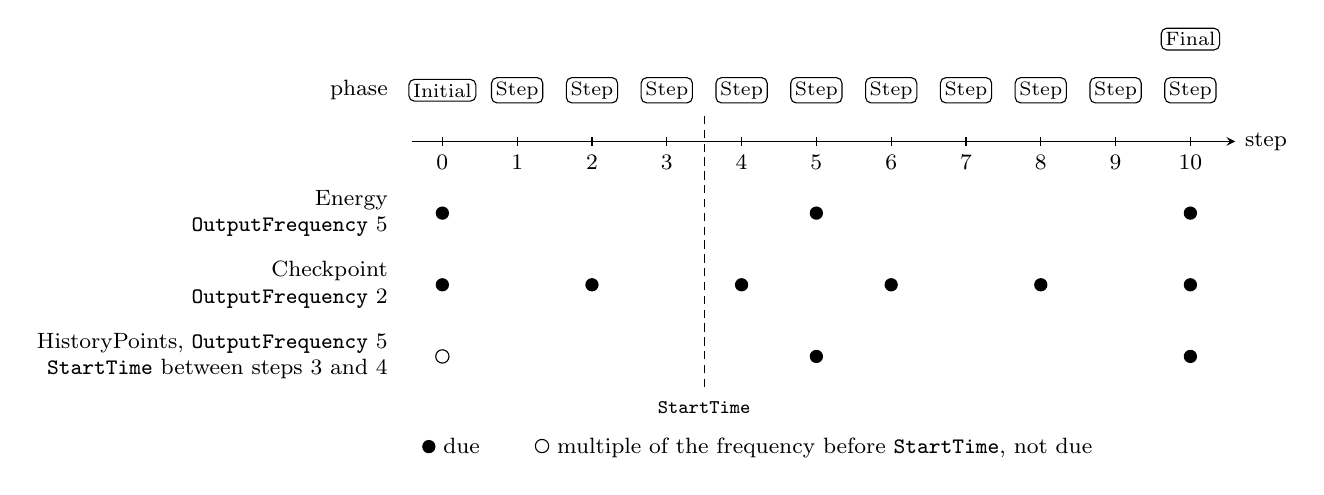
\begin{tikzpicture}[font=\footnotesize, >=stealth, x=0.95cm, y=0.65cm,
    phase/.style={draw, rounded corners=2pt, inner sep=1.5pt, fill=white,
                  font=\scriptsize},
    label/.style={anchor=east, align=right}]
% Axis
\draw[->] (-0.4,0) -- (10.6,0) node[right] {step};
\foreach \s in {0,...,10}
{
    \draw (\s,0.08) -- (\s,-0.08) node[below] {\s};
}

% Phases
\node[label] at (-0.6,1) {phase};
\node[phase] at (0,1) {Initial};
\foreach \s in {1,...,10}
{
    \node[phase] at (\s,1) {Step};
}
\node[phase] at (10,2) {Final};

% Schedules
\newcommand{\schedule}[4]{%
    \node[label] at (-0.6,#1) {#2};
    \foreach \s in {#3}
    {
        \fill (\s,#1) circle (2.4pt);
    }
    \foreach \s in {#4}
    {
        \draw (\s,#1) circle (2.4pt);
    }
}
\schedule{-1.4}{Energy\\ \texttt{OutputFrequency} 5}{0,5,10}{}
\schedule{-2.8}{Checkpoint\\ \texttt{OutputFrequency} 2}{0,2,4,6,8,10}{}
\schedule{-4.2}{HistoryPoints, \texttt{OutputFrequency} 5\\
                \texttt{StartTime} between steps 3 and 4}{5,10}{0}

\draw[densely dashed] (3.5,-4.8) -- (3.5,0.5);
\node[font=\scriptsize] at (3.5,-5.2) {\texttt{StartTime}};

\node[anchor=north west] at (-0.4,-5.6)
    {\tikz\fill (0,0) circle (2.4pt); due \qquad
     \tikz\draw (0,0) circle (2.4pt); multiple of the frequency before
     \texttt{StartTime}, not due};
\end{tikzpicture}%
}
\caption{Filter phases and step schedules. \texttt{RunFilters} runs every
filter at initialisation, after each completed step and at finalisation. A
\texttt{StepSchedule} is due when the global step is a multiple of the
frequency and the time has reached \texttt{StartTime}; the schedules shown
include the initial phase.}
\label{fig:solvercore-filters-schedule}
\end{figure}


\paragraph{Output series and tables.}
\texttt{OutputSeries} creates zero-based numbered paths. Both numbered paths
and backup paths preserve their parent directory; for example,
\texttt{results/run.eny} is backed up as
\texttt{results/run.bak0.eny}. \texttt{RootTableWriter} provides root-only,
RAII-managed whitespace tables with comment metadata, an uncommented column
row, scientific formatting and 16-digit precision. A line is ended with
\texttt{EndRow()}, which flushes it, so each row reaches the file as soon as it
is complete and a run that terminates abnormally keeps every completed row.
HistoryPoints, which writes a row per point at each output step, ends those
rows with a newline and calls \texttt{Flush()} once after the last.

\paragraph{Point sets.}
\texttt{PointSet} parses explicit points, lines, planes and boxes for point
filters. It validates exact arity, finite coordinates, integral point counts
and multiplication overflow before allocating a generated point set.

\subsection{Filter interactions}

\subsubsection{Energy}

Energy obtains the velocity role and constructs \texttt{EnergyOp} with its
component indices. On a due step it requests the velocity gradient from the
shared derived-data cache and passes the underlying velocity field and the
cached gradient to the operator.

The operator supports two- and three-dimensional velocity fields. The
quadrature metric of each block, the quadrature weight times the Jacobian of
every point, is fetched from the data warehouse through
\texttt{LocalRegions::QuadratureMetricKey} the first time a velocity is read
at a given interleave width, laid out as the velocity, so that one storage
index addresses the same point of the velocity, its gradient and the metric at
either width, with no reshape. Each
block is integrated by one \texttt{parallel\_reduce\_sum} over its storage,
on the block's stream, neighbouring threads reading neighbouring entries. It
packs
$\int_\Omega |\mathbf{u}|^2\,d\Omega$, $\int_\Omega |\boldsymbol{\omega}|^2
\,d\Omega$ and the volume into one \texttt{MemoryRegion} and performs a single
reduction to the writer rank. On the writer rank the filter reads the three
values through \texttt{EnergyOp::GetKineticEnergy()}, \texttt{GetEnstrophy()}
and \texttt{GetVolume()}, and writes half of each integral divided by the
volume. Passive scalars are not included.

\subsubsection{Mean}

Mean obtains the registry's physical groups, so that every canonical variable,
including pressure for incompressible flow, is averaged exactly once. For each
group it constructs a \texttt{MeanOp} on the group's own expansion. The
operator reuses the MeanRemoval block operators to accumulate, in the selected
execution space, the integral of every component together with the domain
volume, packs them into one \texttt{MemoryRegion} and reduces them once to the
writer rank. There \texttt{MeanOp::GetMeans()} returns the instantaneous
averages $\int_\Omega f\,d\Omega / \int_\Omega d\Omega$ in component order,
and \texttt{GetVolume()} the volume. The volume is recorded at initialisation
and written to the header. The \texttt{.avg}
table keeps the legacy layout,

\begin{center}
\texttt{\# Time <variables...> volume <V>},
\end{center}

with \texttt{area} in place of \texttt{volume} in two dimensions and one row
per due step, including step zero. Homogeneous, one-dimensional
and embedded-manifold expansions are rejected.

\subsubsection{AeroForces}

AeroForces obtains both velocity and pressure role views and uses the same
cached velocity gradient as Energy. Its operator retains the velocity and
pressure expansions separately, with the component indices of velocity and
pressure in their fields.

During configuration, the operator constructs independent oriented
volume-to-boundary restrictions for pressure and velocity gradient data, so
pressure and velocity expansions do not need identical quadrature. Each
boundary quadrature point has one sparse row per restriction, with a single
entry of weight one where the restriction is a gather. The pressure shares the
blocks of the velocity, as the incompressible solver requires, and the points
on the elements of one block are integrated by one
\texttt{parallel\_reduce\_sum} of the twelve sums on the block's stream,
whatever the shapes of its faces. The rows are gathered on the host at
configuration. The first time the gradient is read at an interleave width, one
or the width of the execution space, the rows of each block are copied to the
operator's memory space for that width: the restriction sources are converted
to storage offsets, those of the pressure at both widths, and the points are
ordered by the offset of their first gradient source, so that neighbouring
threads read neighbouring entries where the boundary allows; the normals and
moment arms are stored point-minor for the same reason. \texttt{Apply()} then
reads the pressure and the gradient where they are stored, at either width. The
operator integrates pressure and viscous forces and moments into twelve packed
values and reduces them to the writer rank. There the filter reads the four
Cartesian 3-vectors through \texttt{AeroForcesOp::GetPressureForce()},
\texttt{GetViscousForce()}, \texttt{GetPressureMoment()} and
\texttt{GetViscousMoment()}; in two dimensions the $z$ force components and
the $x$ and $y$ moment components are zero.

The filter validates that the boundary selection is non-empty and contains no
duplicates, and that every selected boundary identifier exists on some rank.
Directions and pivot points require exactly three finite values; directions are
normalised but are not required to be mutually orthogonal. Output retains
separate pressure, viscous and total columns.

\subsubsection{HistoryPoints}

HistoryPoints obtains the registry's physical groups so every canonical
variable is sampled once. At initialisation, an interpolation operator for each
registered layout determines containing elements and interpolation weights.
Point ownership is resolved with a maximum-rank reduction, giving deterministic
highest-rank ownership when a point lies on a partition boundary. A point that
cannot be found on any rank produces an explicit diagnostic.

At each output step each group is evaluated locally, block by block on the
blocks' streams, one point per thread. The storage offset of the element
holding each point is built the first time a field is read at an interleave
width, one or the width of the execution space, which is a template parameter
of the kernel, and the points of a block are sorted by element, so that at the execution
space's width neighbouring threads read neighbouring lanes. The values are then
collected on the writer rank by one sum over the ranks: each point is owned by
one rank, and every other rank contributes zero. On the writer rank \texttt{HistoryPointsOp::GetValues()} returns each
group's values point-major, with component \texttt{comp} of point
\texttt{point} at \texttt{point * nComp + comp}, and the groups are
interleaved into one point-major table, whose schema is

\begin{center}
\texttt{Time Point <variables...>}.
\end{center}

Single-file histories and zero-based numbered snapshots use the same scheduling
and output-series utilities.

\subsubsection{Checkpoint}

Checkpoint does not need to inspect a field view. When its schedule is due, it
updates \texttt{FilterFileNum} through the metadata service, obtains the next
zero-based filename from \texttt{OutputSeries}, and calls
\texttt{writeFields}. This establishes the same step and numbering semantics as
the other output filters.

\subsection{Integration with redesigned equation systems}

The registry is also the compatibility boundary for ADRSolverRedesign and
CompressibleFlowSolverRedesign. An equation system should publish mathematical
meaning, rather than relying on a filter to interpret the ordering of its
stored variables. This is especially important because the three solver
families store different states:

\begin{center}
\begin{tabularx}{\textwidth}{lXX}
\hline
Solver & canonical solution & additional semantic roles \\
\hline
ADRSolverRedesign & transported scalar fields & none by default \\
IncNavierStokesSolverRedesign & velocity and passive scalars & velocity,
pressure \\
CompressibleFlowSolverRedesign & density, momentum and total energy & derived
velocity, pressure and density \\
\hline
\end{tabularx}
\end{center}

\paragraph{Generic output filters.}
The default \texttt{EquationSystem::v\_GetFieldRegistry()} publishes
\texttt{m\_fields} as the solution role and as one non-overlapping physical
group, and installs \texttt{v\_GetOutputFieldViews()} as the lazy coefficient
provider. Consequently, unsteady ADR and compressible equation systems inherit
the data contract required by Checkpoint and HistoryPoints.
Their history files contain the solver's canonical variables: transported
variables for ADR and conservative variables for compressible flow.

The equation system's output path must be retained when overriding this
provider. Continuous fields use the global forward transform, whereas
discontinuous fields use \texttt{ProjectPhysToCoeffs()}, the element-local
$L^2$ projection that makes DG restarts exact. Returning stale
\texttt{m\_fields\_coeff} storage would make checkpoints incorrect even though
the files themselves are structurally valid.

\paragraph{Incompressible flow.}
VelocityCorrectionScheme overrides the registry because pressure has separate
storage and may have a different expansion. It publishes velocity as the first
\texttt{spaceDimension} components of the solution field, publishes pressure
as a separate role, and retains passive scalars only in the canonical solution
group. This is the complete contract for the filters described here.

\paragraph{ADR.}
The ADR solution represents transported quantities, not fluid momentum. Its
prescribed advection field is an operator coefficient and must not
automatically be advertised as the velocity whose kinetic energy is measured.
Checkpoint and HistoryPoints are therefore meaningful through the default
registry. Energy and AeroForces should report a missing-role
diagnostic. If a future coupled ADR system has genuine fluid state, that
equation system can explicitly publish velocity, pressure and stress roles;
the generic scalar ADR solver should not invent them.

SteadyADR currently derives directly from \texttt{EquationSystem}, while the
filter lifecycle is driven by \texttt{UnsteadySystem}. Supporting filters for
a steady solve therefore also requires moving the lifecycle driver to a common
equation-system or driver hook and defining whether the single solved state is
an initial, step-zero or final event. This is independent of field-registry
compatibility.

\paragraph{Compressible flow.}
The compressible solution is conservative, so component slices of
\texttt{m\_fields} cannot be used as velocity or pressure views. Full support
requires the compressible equation system to provide backend-native primitive
workspaces and populate

\begin{itemize}
\item velocity as momentum divided by density;
\item pressure through the configured equation of state; and
\item density for density-weighted diagnostics.
\end{itemize}

These values should be computed lazily once per filter phase and shared by all
consumers. A natural extension is a lazy physical-role provider in
\texttt{FieldRegistry}, with the resolved view cached for the lifetime of that
registry. The conversion kernel and its workspace belong to the compressible
solver (or to a compressible primitive-state service), not to Energy or
AeroForces. This preserves the backend-independent filter layer and avoids a
host conversion of conservative fields.

Energy additionally needs an explicit weighting policy. The current operator
implements constant-density incompressible kinetic energy and enstrophy. To
match the legacy fluid interface for variable-density flow, its operator must
accept the density role and integrate density-weighted quantities. The
unweighted incompressible path should remain available without allocating a
unit-density field.

AeroForces requires a constitutive contract as well as primitive pressure.
The current viscous term assumes the incompressible constant-viscosity stress.
Compressible Navier--Stokes may use dynamic, possibly temperature-dependent,
viscosity and a dilatational stress term; Euler flow has no viscous traction.
The portable interface should therefore publish a viscous-stress (or boundary
traction) view/service computed by the equation system's diffusion model.
AeroForces can then combine this with pressure using its independent boundary
restrictions. Treating momentum gradients as velocity gradients, or reusing
the incompressible Reynolds-number formula, would be incorrect.

\paragraph{Capability validation and tests.}
Filters should continue to validate their required roles during
initialisation. Generic filters require solution/physical/coefficient groups;
Energy requires velocity and optionally density according to its weighting
mode; AeroForces requires pressure plus velocity/stress capabilities. Missing
capabilities are configuration errors with the equation-system and filter
names in the diagnostic.

The cross-solver regression matrix should exercise Checkpoint and
HistoryPoints for unsteady ADR, incompressible flow and compressible flow,
including numerical restart contents for both CG and DG layouts.
Compressible Energy tests need analytic variable-density fields, and
compressible AeroForces tests need inviscid and viscous cases using the same
equation-of-state and transport models as the solver. Negative tests should
confirm that ADR rejects fluid-only filters and that Euler rejects a requested
viscous contribution.

\subsection{Differences from the legacy filter interface}

The principal changes relative to the SolverUtils filters, and to the
Checkpoint filter SolverCore had before this interface, are as follows.

\begin{itemize}
\item Filters previously stored a weak pointer to \texttt{EquationSystem} and
      queried fields, metadata and output methods directly. They now receive
      explicit per-phase capabilities through \texttt{FilterContext}.
\item Lifecycle methods previously received only the time. The new context also
      carries the actual integration step and explicit initial/final flags.
      The unused \texttt{IsTimeDependent} and mutable
      \texttt{SetApplyOnInitialise} APIs have been removed.
\item Filters previously maintained local call counters, so the meaning of a
      frequency depended on when the filter was invoked. Stateless schedules
      now use the global integration step.
\item Energy and AeroForces share one physical-derivative operator and
      gradient field through the derived-data cache, instead of each owning
      its own.
\item Result operators reduce their packed results to the writer rank only,
      through a device-aware \texttt{Comm::Reduce} overload for
      \texttt{MemoryRegion}. GPU-aware MPI uses device storage; other MPI
      configurations stage through the MemoryRegion host representation.
      As for the norm operators, \texttt{Apply()} returns nothing and the
      filter reads the reduced values on the writer rank through the
      operator's getters, which copy them to the host.
\item AeroForces supports pressure and velocity expansions with different
      volume quadrature, through independent restriction maps, and validates
      its boundary identifiers rather than silently ignoring unknown ones.
\item Parameter parsing, text output, numbered paths and backups were
      implemented independently in each filter. They now use common utilities,
      making malformed input and output naming consistent across filter types.
\end{itemize}

The resulting boundary is intentionally narrow: equation systems publish
meaningful state and controlled services, while filters own only their static
configuration and persistent diagnostic state. High-level filter logic remains
independent of Serial, SIMD, CUDA and HIP backends; backend-specific evaluation
continues to live in the operator layer.
